\section{Formatting detectors outputs}
In the previous chapter, we were able to extract the features and the packer used for each piece of malware before uploading them in a database. At this point, they are stored in raw format, i.e. no formatting was done yet. This is the purpose of this section. 

The problem that we have to deal with comes from the output of the detectors, namely the name of the packer. It can be articulated in three points:
\begin{itemize}
    \item  As the packer names are just strings of characters, it becomes more difficult to compare them with each other. Typography renders two different results for the computer whereas in our eyes they are identical, and this because of a simple space between two letters, an upper-case, the character \textit{i} instead of the number \textit{1}...  For example, the outputs "petite" and "P3TITE" will be evaluated as two different strings although they both indicate the use of the PEtite packer. 
    \item The previous problem presented the difficulty of comparing two results from two different detectors, but the problem also arises when comparing the results of the same detector. Very often it returns not only the name of the packer used but also its version. In our experiments, we do not care about the version used, "UPX 2.24" and "upx 1.0" need to be grouped in one single "upx" packer.
    \item A big issue is that these different typefaces and versions cannot be detected before the malware are actually scanned. In addition, new versions as well as new packers are released every day, increasing the difficulty to build realistic datasets, as stated by Hubbabilli and Dogra \cite{hubballi_detecting_2016} and Biondi et al. \cite{biondi_effective_2019}. Moreover, if a new detector is added to our system, there is a good chance that we will have even more new output formats. 
\end{itemize}

To solve this issue, before generating our ground truths for the machine learning algorithms, we apply a set of renaming rules to the malware. The packers are first converted to lowercase. Then, we apply a series of aliases. All this together, an initial string such as "UPX(3.94)[NRV,raw]", when cleaned, is eventually renamed in "upx". For results that do not correspond to any packer, such as linkers or compilers, they are renamed in "none", which is the value given to malware that are not packed.

To generate the renaming rules, we added a tab on our web interface. On this page, the list of packers that were not yet met and therefore not yet processed is displayed. Next to each name stands a form where the name of the packer can be changed. If it appears that the entry is not a packer, one should write the value "none" instead. Once cleaned, the initial packer will never be displayed again in this menu. Figure \ref{fig:cleaning} shows a screenshot of the renaming tab from the website.

\begin{figure}[!htb]
\centering
  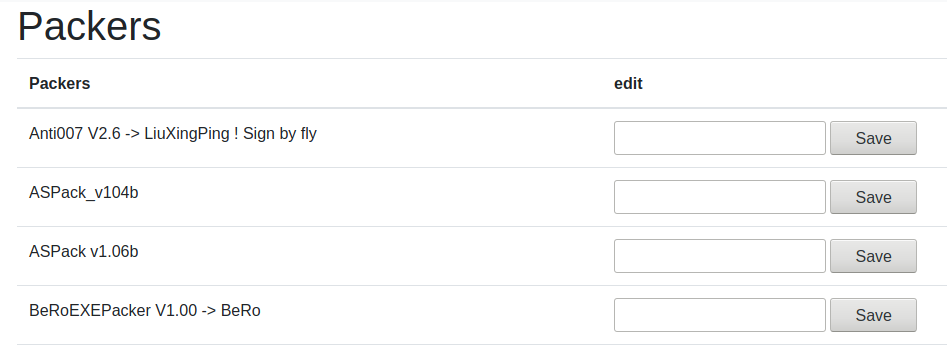
\includegraphics[width=\linewidth]{Figures/cleaning.png}
  \caption{Renaming forms}
  \label{fig:cleaning}
\end{figure}

The rules that are generated by indicating the correct packer name are saved in the database to be applied to current and future malware as well and are available through in the website via another tab. At the beginning of May 2020, we had already encoded a little more than 1200 rules.

To effectively apply all these renaming rules before performing a dump, the \textit{clean.py} script needs to be run, which will apply all changes to the database. A strong requirement is therefore to check beforehand on the website that no unknown packer are left and that they have been renamed properly.